\documentclass[a4paper, 12pt]{article}

\usepackage{amsmath}
\usepackage{graphicx}

\begin{document}
	
	\pagenumbering{arabic}
	\title{Surface Area of Spheres - the Wok Problem}
		\author{Nick Wang}
		\date{\today}
	\maketitle
	
	\section{Introduction}
		Since the first introduction to geometry in elementary school, students have investigated the volume, surface area, and many other geometric properties of 2-Dimensional,as well as 3-Dimensional shapes. Yet one area the students' understanding falls apart is circles and spheres. As a part of the curriculum of second year Calculus students, today we look at one of these problems and approach from a Calculus point of view:\\
		\begin{center}
			\textit {One such problem states that a semi-spherical wok exists with diameter of 16 cm and height 9 cm. We are to paint the outside and inside of 5000 woks with 0.5 mm thick of paint each. Calculate the volume of paint needed in liters. }\\
		\end{center}
		\begin{figure}[h]
			\centering
			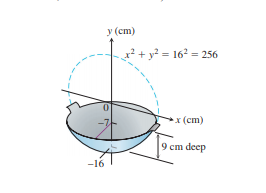
\includegraphics[width=0.5\textwidth]{wok.png}
			\caption{Wok Dimensions}
		\end{figure}
	
	\section{Interpolating the Problem}
		\label{interpolation}
		The problem states that a wok needs to be painted on both its inside and outside. This meant the area of paint needed is the surface area of the wok's inside and outside. Upon closer inspection we realize the paint is painted at 0.5 mm thick, which meant the volume of paint needed on each side is the surface area multiplied by the height of the paint, which is 0.5 mm. This meant the  real question this question is asking is what is the surface area of part of a sphere.\\\\
		Realizing this we can use the equation $A = \int2\pi y\sqrt{1^2+\frac{dy}{dx})^2}dx$ to calculate surface area. Thus we need to find f'(x) with given equation $$x^2+y^2=256$$Furthermore since the wok represents part of a sphere, we can naturally rotate the sphere onto the x-axis for easier calculation. Thus simplifying we get:$$y=\sqrt{256-x^2}$$
	\section{Calculations} 
		Using equations we got from section \ref{interpolation}: $$\frac{dy}{dx}=\frac{1}{2}{(256-x^2)}^{-1/2} 2x$$
		Plugging in the equation and the bounds:$$A = \int_7^{16} 2\pi \sqrt{256-x^2}\sqrt{1^2+{(\frac{1}{2}{(256-x^2)}^{-1/2} 2x)}^2}dx$$
		Expanding each term:$$A =2\pi \int_7^{16} \sqrt{256-x^2}\sqrt{1+{(256-x^2)}^{-1} x^2}dx$$
		Changing negative exponent to a fraction:$$A =2\pi \int_7^{16} \sqrt{256-x^2}\sqrt{1+\frac{x^2}{256-x^2}}dx$$
		Rewriting 1 with common denominator:$$A =2\pi \int_7^{16} \sqrt{256-x^2}\sqrt{\frac{256-x^2+x^2}{256-x^2}}dx$$
		Canceling out similar terms and pulling out constant 256:$$A =2\pi \int_7^{16} 16\sqrt{256-x^2} \sqrt{\frac{1}{256-x^2}}dx$$
		Moving the constants out of the integral and simplifying the integrand:$$A =32\pi \int_7^{16}{(256-x^2)}^{1/2} {(256-x^2)}^{-1/2}dx$$
		Combining similar terms:$$A =32\pi \int_7^{16}{(256-x^2)}^{1/2-1/2} dx$$
		Simplifying the integrand:$$A =32\pi \int_7^{16}1 dx$$
		Taking the integral:$$A =32\pi \left[x\right]_7^{16}$$
		Plugging in the bounds:$$A =32\pi {(16-7)}=288\pi$$
		Thus we have found the surface area of one side of the wok in $cm^2$. To calculate the total volume of paint needed, we multiply the surface area. In order to convert final result to liters, we use dimensional analysis:$$V=\frac{288\pi cm^2}{1 side}\cdot\frac{ 0.5 mm}{1 side} \cdot\frac{1 cm}{10 mm}\cdot\frac{1 side}{1 wok}\cdot5000 wok\cdot\frac{1 liter}{1000cm^3}=72\pi/side$$\\
		Thus to paint 5000 woks of this dimension we need $72\pi$ liters of paint for each side of the wok.

\end{document}